\chapter{Model 1: Re-evaluation of Model 5b with 2024 Data}\label{ch:model1}

% Load model-specific values
% Model 1 Calibrated Values
% Generated: 2025-10-02 01:58:23.185499
% Model: Linear with Outlier Removal

% Core Metrics
\renewcommand{\ModelOneRSquaredTrain}{0.2383}
\renewcommand{\ModelOneRSquaredTest}{0.2178}
\renewcommand{\ModelOneRMSETrain}{39,238}
\renewcommand{\ModelOneRMSETest}{39,500}
\renewcommand{\ModelOneMAETrain}{27,831}
\renewcommand{\ModelOneMAETest}{27,912}
\renewcommand{\ModelOneMAPETrain}{85.2}
\renewcommand{\ModelOneMAPETest}{84.8}
\renewcommand{\ModelOneCVMean}{0.2372}
\renewcommand{\ModelOneCVStd}{0.0196}
\renewcommand{\ModelOneWithinOneK}{2.4}
\renewcommand{\ModelOneWithinTwoK}{4.9}
\renewcommand{\ModelOneWithinFiveK}{15.8}
\renewcommand{\ModelOneWithinTenK}{28.5}
\renewcommand{\ModelOneWithinTwentyK}{49.5}
\renewcommand{\ModelOneTrainingSamples}{27,339}
\renewcommand{\ModelOneTestSamples}{6,834}

% Subgroup Metrics
\renewcommand{\ModelOneSubgrouplivingFHN}{5,941}
\renewcommand{\ModelOneSubgrouplivingFHRSquared}{0.222}
\renewcommand{\ModelOneSubgrouplivingFHRMSE}{39,928}
\renewcommand{\ModelOneSubgrouplivingFHBias}{-7,487}
\renewcommand{\ModelOneSubgrouplivingILSLN}{893}
\renewcommand{\ModelOneSubgrouplivingILSLRSquared}{0.179}
\renewcommand{\ModelOneSubgrouplivingILSLRMSE}{36,524}
\renewcommand{\ModelOneSubgrouplivingILSLBias}{-3,272}
\renewcommand{\ModelOneSubgroupageAgeUnderTwentyOneN}{694}
\renewcommand{\ModelOneSubgroupageAgeUnderTwentyOneRSquared}{0.138}
\renewcommand{\ModelOneSubgroupageAgeUnderTwentyOneRMSE}{34,649}
\renewcommand{\ModelOneSubgroupageAgeUnderTwentyOneBias}{-8,152}
\renewcommand{\ModelOneSubgroupageAgeTwentyOneToThirtyN}{1,797}
\renewcommand{\ModelOneSubgroupageAgeTwentyOneToThirtyRSquared}{0.161}
\renewcommand{\ModelOneSubgroupageAgeTwentyOneToThirtyRMSE}{44,751}
\renewcommand{\ModelOneSubgroupageAgeTwentyOneToThirtyBias}{-7,785}
\renewcommand{\ModelOneSubgroupageAgeThirtyOnePlusN}{4,343}
\renewcommand{\ModelOneSubgroupageAgeThirtyOnePlusRSquared}{0.218}
\renewcommand{\ModelOneSubgroupageAgeThirtyOnePlusRMSE}{37,876}
\renewcommand{\ModelOneSubgroupageAgeThirtyOnePlusBias}{-6,391}
\renewcommand{\ModelOneSubgroupcostQOneLowN}{1,709}
\renewcommand{\ModelOneSubgroupcostQOneLowRSquared}{-10.000}
\renewcommand{\ModelOneSubgroupcostQOneLowRMSE}{31,272}
\renewcommand{\ModelOneSubgroupcostQOneLowBias}{+24,162}
\renewcommand{\ModelOneSubgroupcostQTwoN}{1,708}
\renewcommand{\ModelOneSubgroupcostQTwoRSquared}{-6.029}
\renewcommand{\ModelOneSubgroupcostQTwoRMSE}{20,461}
\renewcommand{\ModelOneSubgroupcostQTwoBias}{+9,755}
\renewcommand{\ModelOneSubgroupcostQThreeN}{1,708}
\renewcommand{\ModelOneSubgroupcostQThreeRSquared}{-4.117}
\renewcommand{\ModelOneSubgroupcostQThreeRMSE}{26,401}
\renewcommand{\ModelOneSubgroupcostQThreeBias}{-13,739}
\renewcommand{\ModelOneSubgroupcostQFourHighN}{1,709}
\renewcommand{\ModelOneSubgroupcostQFourHighRSquared}{-2.230}
\renewcommand{\ModelOneSubgroupcostQFourHighRMSE}{64,390}
\renewcommand{\ModelOneSubgroupcostQFourHighBias}{-47,917}

% Variance Metrics
\renewcommand{\ModelOneCVActual}{1.010}
\renewcommand{\ModelOneCVPredicted}{0.692}
\renewcommand{\ModelOnePredictionInterval}{152,432}
\renewcommand{\ModelOneBudgetActualCorr}{0.498}
\renewcommand{\ModelOneQuarterlyVariance}{87.9}
\renewcommand{\ModelOneAnnualAdjustmentRate}{92.4}

% Population Scenarios
\renewcommand{\ModelOnePopcurrentbaselineClients}{32,188}
\renewcommand{\ModelOnePopcurrentbaselineAvgAlloc}{37,280}
\renewcommand{\ModelOnePopcurrentbaselineWaitlistChange}{+0}
\renewcommand{\ModelOnePopcurrentbaselineWaitlistPct}{+0.0}
\renewcommand{\ModelOnePopmodelbalancedClients}{32,831}
\renewcommand{\ModelOnePopmodelbalancedAvgAlloc}{36,534}
\renewcommand{\ModelOnePopmodelbalancedWaitlistChange}{+643}
\renewcommand{\ModelOnePopmodelbalancedWaitlistPct}{+2.0}
\renewcommand{\ModelOnePopmodelefficiencyClients}{33,797}
\renewcommand{\ModelOnePopmodelefficiencyAvgAlloc}{35,416}
\renewcommand{\ModelOnePopmodelefficiencyWaitlistChange}{+1,609}
\renewcommand{\ModelOnePopmodelefficiencyWaitlistPct}{+5.0}
\renewcommand{\ModelOnePopcategoryfocusedClients}{27,359}
\renewcommand{\ModelOnePopcategoryfocusedAvgAlloc}{43,990}
\renewcommand{\ModelOnePopcategoryfocusedWaitlistChange}{-4,828}
\renewcommand{\ModelOnePopcategoryfocusedWaitlistPct}{-15.0}
\renewcommand{\ModelOnePoppopulationmaximizedClients}{37,016}
\renewcommand{\ModelOnePoppopulationmaximizedAvgAlloc}{32,434}
\renewcommand{\ModelOnePoppopulationmaximizedWaitlistChange}{+4,828}
\renewcommand{\ModelOnePoppopulationmaximizedWaitlistPct}{+15.0}

% Model 1 Specific Metrics
\renewcommand{\ModelOneOutliersRemoved}{2570}
\renewcommand{\ModelOneOutlierPercentage}{9.4}
\renewcommand{\ModelOneTransformation}{Square Root}
\renewcommand{\ModelOneNumFeatures}{26}
\renewcommand{\ModelOnePredictionFloor}{5,000}

% Feature Selection Specific Values
\renewcommand{\ModelOneFeatureSelection}{True}
\renewcommand{\ModelOneFiscalYears}{2024}
\renewcommand{\ModelOneMIScoreTop}{0.272}
\renewcommand{\ModelOneVarianceExplained}{89.0}


% Setup template to use Model 1's commands
\SetupModelTemplate{One}  % Just call the macro, don't input the file again. It is loaded in 0config.tex

% Store model number for template
\def\themodel{1}

\section{Executive Summary}

Model 1 represents a \textbf{direct re-evaluation of Model 5b} (Tao \& Niu 2015) using fiscal year 2024 data. This model maintains the EXACT feature specification from Model 5b to enable direct performance comparison across the 9-year period from 2015 to 2024.

\subsection{Purpose and Scope}

The primary objective of Model 1 is to answer a critical question: \textit{Does Model 5b, which performed exceptionally well with FY2013--2014 data ($R^2$ = \ModelOneFiveBRSquaredTwoThousandFifteen), maintain its predictive power with 2024 data?} By preserving the exact same 21 features, transformation, and outlier detection methodology, we can isolate temporal changes in model performance from methodological changes.

\subsection{Key Findings}

\begin{itemize}
    \item \textbf{Original Model 5b (2015)}: Test $R^2$ = \ModelOneFiveBRSquaredTwoThousandFifteen, RMSE = \$\ModelOneFiveBRMSETwoThousandFifteen{} (sqrt scale), Outliers = \ModelOneFiveBOutlierPctTwoThousandFifteen\%
    \item \textbf{Model 1 Re-evaluation (2024)}: Test $R^2$ = \MRSquaredTest, RMSE = \$\MRMSETest, Outliers = \MOutlierPct\%
    \item \textbf{Performance Change}: $\Delta$$R^2$ = \ModelOneRSquaredDeltaFromTwoThousandFifteen
    \item \textbf{Feature Specification}: Identical 21 features as Model 5b
    \item \textbf{Cross-Validation}: Mean $R^2$ = \MCVMean{} ± \MCVStd
    \item \textbf{Sample Size}: \MTrainingSamples{} training, \MTestSamples{} test
\end{itemize}

\section{Historical Context: Model 5b (Tao \& Niu 2015)}

\subsection{Original Development}

Model 5b was developed by Tao and Niu during 2014--2015 as part of a comprehensive evaluation of statistical models for the Florida iBudget algorithm. The model was trained on FY2013--2014 claims data and represented the culmination of extensive model selection and validation work.

\textbf{Model 5b Performance (2015):}
\begin{itemize}
    \item Test $R^2$: \ModelOneFiveBRSquaredTwoThousandFifteen{} (explains 80\% of cost variance)
    \item Residual Standard Error: \$\ModelOneFiveBRMSETwoThousandFifteen{} (in sqrt-transformed scale)
    \item Schwarz Bayesian Criterion (SBC): \ModelOneFiveBSBCTwoThousandFifteen
    \item Training Sample: 23,215 consumers (after outlier removal)
    \item Outliers Removed: 2,410 (\ModelOneFiveBOutlierPctTwoThousandFifteen\% of 25,625 consumers)
\end{itemize}

\subsection{Why Model 5b Was Selected}

Among numerous candidate models evaluated by Tao and Niu, Model 5b was chosen as the recommended model for the following reasons:

\begin{enumerate}
    \item \textbf{Superior Predictive Performance}: Highest $R^2$ among models tested
    \item \textbf{Feature Parsimony}: 21 carefully selected features (balance between completeness and interpretability)
    \item \textbf{Theoretical Justification}: Features aligned with regulatory requirements and clinical understanding
    \item \textbf{Interaction Terms}: Innovative inclusion of interaction terms captured how support needs vary by living setting
    \item \textbf{Robust Outlier Detection}: Studentized residuals method provided statistically principled outlier removal
    \item \textbf{Regulatory Compliance}: Transparent, interpretable, and consistent with F.S. 393.0662 requirements
\end{enumerate}

\section{Model Specification}

\subsection{Mathematical Formulation}

Model 5b uses ordinary least squares regression with square-root transformation of the dependent variable:

\begin{equation}\label{eq:model5b}
\sqrt{y_i} = \beta_0 + \sum_{j=1}^{21} \beta_j x_{ij} + \epsilon_i, \quad \epsilon_i \sim N(0, \sigma^2)
\end{equation}

where:
\begin{itemize}
    \item $y_i$ = total annual cost for consumer $i$ (in dollars)
    \item $x_{ij}$ = feature $j$ for consumer $i$ ($j = 1, \ldots, 21$)
    \item $\beta_0$ = intercept
    \item $\beta_j$ = coefficient for feature $j$
    \item $\epsilon_i$ = random error term
\end{itemize}

\textbf{Back-transformation to original scale:}
\begin{equation}
\hat{y}_i = \left(\hat{\beta}_0 + \sum_{j=1}^{21} \hat{\beta}_j x_{ij}\right)^2
\end{equation}

\subsection{Feature Selection (21 Features)}

Model 5b uses exactly \ModelOneNumFeatures{} features, organized into five categories:

\subsubsection{1. Living Settings (5 Dummy Variables)}

\begin{table}[h]
\centering
\caption{Living Setting Features (Reference Category: Family Home)}
\begin{tabular}{lll}
\toprule
\textbf{Feature} & \textbf{Description} & \textbf{Coding} \\
\midrule
LiveILSL & Independent/Supported Living & 1 if ILSL, 0 otherwise \\
LiveRH1 & Residential Habilitation Level 1 & 1 if RH1, 0 otherwise \\
LiveRH2 & Residential Habilitation Level 2 & 1 if RH2, 0 otherwise \\
LiveRH3 & Residential Habilitation Level 3 & 1 if RH3, 0 otherwise \\
LiveRH4 & Residential Habilitation Level 4 & 1 if RH4, 0 otherwise \\
\bottomrule
\end{tabular}
\end{table}

\textbf{Design Decision:} Family Home (FH) serves as the reference category. This means all living setting coefficients represent the additional cost associated with that setting compared to family home care.

\subsubsection{2. Age Groups (2 Dummy Variables)}

\begin{table}[h]
\centering
\caption{Age Group Features (Reference Category: Ages 3--20)}
\begin{tabular}{lll}
\toprule
\textbf{Feature} & \textbf{Description} & \textbf{Coding} \\
\midrule
Age21\_30 & Ages 21--30 & 1 if age 21--30, 0 otherwise \\
Age31Plus & Ages 31 and older & 1 if age 31+, 0 otherwise \\
\bottomrule
\end{tabular}
\end{table}

\textbf{Design Decision:} Ages 3--20 serve as the reference category. This captures the transition from pediatric to adult services and the stability of support needs in adulthood.

\subsubsection{3. Behavioral Sum (1 Variable)}

\textbf{BSum}: Sum of behavioral support needs from Quality of Support Index (QSI) items related to behavioral challenges. Higher values indicate greater behavioral support needs.

\subsubsection{4. Interaction Terms (3 Variables) --- CRITICAL}

These are Model 5b's key innovation, capturing how functional and behavioral needs interact with living settings:

\begin{itemize}
    \item \textbf{FHFSum} = (Family Home indicator) × (Functional Sum)
        \begin{itemize}
            \item Captures how functional needs translate to costs in family home settings
            \item Positive coefficient indicates additional functional support costs in family homes
        \end{itemize}
    
    \item \textbf{SLFSum} = (Supported Living indicator) × (Functional Sum)
        \begin{itemize}
            \item Captures how functional needs translate to costs in supported living
            \item Typically larger coefficient than FHFSum (more intensive support model)
        \end{itemize}
    
    \item \textbf{SLBSum} = (Supported Living indicator) × (Behavioral Sum)
        \begin{itemize}
            \item Captures how behavioral challenges affect costs in supported living
            \item Critical for appropriate resource allocation for complex behavioral needs
        \end{itemize}
\end{itemize}

\textbf{Interpretation Example:} If SLFSum has coefficient 2.05 and FHFSum has coefficient 0.63 (as in original Model 5b), this means each unit increase in functional needs costs an additional \$2.05 in supported living settings but only \$0.63 in family home settings. This reflects the different care models and support intensity.

\subsubsection{5. QSI Questions (10 Variables)}

Selected Quality of Support Index items that proved most predictive in the original model selection process:

\begin{table}[h]
\centering
\caption{Selected QSI Questions (From Model 5b)}
\begin{tabular}{ll}
\toprule
\textbf{Question} & \textbf{Domain} \\
\midrule
Q16 & Eating \\
Q18 & Transfers \\
Q20 & Hygiene \\
Q21 & Dressing \\
Q23 & Self-protection \\
Q28 & Inappropriate Sexual Behavior \\
Q33 & Injury to Person/Property \\
Q34 & Use of Restraints \\
Q36 & Use of Psychotropic Medications \\
Q43 & Treatment (Physician Prescribed) \\
\bottomrule
\end{tabular}
\end{table}

\subsection{Outlier Detection: Studentized Residuals}

Model 5b uses studentized residuals to identify outliers:

\begin{equation}
t_i = \frac{\hat{\epsilon}_i}{\hat{\sigma}\sqrt{1 - h_{ii}}}
\end{equation}

where:
\begin{itemize}
    \item $\hat{\epsilon}_i$ = residual for observation $i$
    \item $\hat{\sigma}$ = estimated standard deviation of residuals
    \item $h_{ii}$ = leverage (diagonal element of hat matrix $H = X(X'X)^{-1}X'$)
\end{itemize}

\textbf{Outlier Criterion:} Observations with $|t_i| \geq 1.645$ are removed. This corresponds to approximately 10\% removal (5\% in each tail of the $N(0,1)$ distribution).

\textbf{Advantage:} Unlike simple percentile-based removal, studentized residuals account for leverage, preventing high-influence observations from masking as good fits simply because they pull the regression line toward themselves.

\section{Comparison: Model 5b (2015) vs.\ Model 1 (2024)}

\begin{table}[h]
\centering
\caption{Model 5b Performance: 2015 vs.\ 2024}
\begin{tabular}{lcc}
\toprule
\textbf{Metric} & \textbf{Model 5b (2015)} & \textbf{Model 1 (2024)} \\
\midrule
$R^2$ & \ModelOneFiveBRSquaredTwoThousandFifteen & \MRSquaredTest \\
RMSE & \$\ModelOneFiveBRMSETwoThousandFifteen{} (sqrt) & \$\MRMSETest{} (original) \\
SBC & \ModelOneFiveBSBCTwoThousandFifteen & \ModelOneSBC \\
Sample Size & 23,215 & \MTrainingSamples \\
Outliers Removed & \ModelOneFiveBOutlierPctTwoThousandFifteen\% & \MOutlierPct\% \\
\midrule
\textbf{Change ($\Delta$)} & \textbf{---} & \textbf{---} \\
$\Delta$$R^2$ & --- & \ModelOneRSquaredDeltaFromTwoThousandFifteen \\
$\Delta$SBC & --- & \ModelOneSBCDeltaFromTwoThousandFifteen \\
$\Delta$Outlier\% & --- & \ModelOneOutlierPctDeltaFromTwoThousandFifteen\% \\
\bottomrule
\end{tabular}
\end{table}

\textbf{Interpretation:}
\begin{itemize}
    \item \textbf{$\Delta$$R^2$}: Change in explained variance. Negative values indicate declining predictive power; positive values indicate improvement.
    \item \textbf{$\Delta$SBC}: Change in model complexity penalty. Lower (more negative) is better. Positive delta suggests the model is less parsimonious with 2024 data.
    \item \textbf{$\Delta$Outlier\%}: Change in percentage of outliers. Large changes may indicate distributional shifts in the population or cost structure.
\end{itemize}

% ============================================
% INSERT UNIVERSAL TEMPLATE HERE
% ============================================
% ============================================
% model_template.tex
% ============================================
% Universal template for all models
% Uses generic \M... commands that get mapped to model-specific commands
% 
% IMPORTANT: Call \SetupModelTemplate{ModelWord} BEFORE inputting this file
% ============================================

\section{Performance Metrics}

\subsection{Overall Performance}

\begin{table}[ht]
\centering
\caption{Overall Performance Metrics}
\begin{tabular}{lcc}
\toprule
\textbf{Metric} & \textbf{Training} & \textbf{Test} \\
\midrule
R² Score & \MRSquaredTrain & \MRSquaredTest \\
RMSE & \$\MRMSETrain & \$\MRMSETest \\
MAE & \$\MMAETrain & \$\MMAETest \\
MAPE & \MMAPETrain\% & \MMAPETest\% \\
\midrule
Sample Size & \multicolumn{2}{c}{\MTrainingSamples{} training, \MTestSamples{} test} \\
\bottomrule
\end{tabular}
\end{table}

\subsection{Accuracy Bands}

\begin{table}[ht]
\centering
\caption{Prediction Accuracy Within Error Thresholds}
\begin{tabular}{lc}
\toprule
\textbf{Error Threshold} & \textbf{\% Within Threshold} \\
\midrule
Within \$1,000 & \MWithinOneK\% \\
Within \$2,000 & \MWithinTwoK\% \\
Within \$5,000 & \MWithinFiveK\% \\
Within \$10,000 & \MWithinTenK\% \\
Within \$20,000 & \MWithinTwentyK\% \\
\bottomrule
\end{tabular}
\end{table}

\subsection{Cross-Validation Results}

\begin{table}[ht]
\centering
\caption{10-Fold Cross-Validation Performance}
\begin{tabular}{lc}
\toprule
\textbf{Metric} & \textbf{Value} \\
\midrule
Mean R² & \MCVMean \\
Standard Deviation & \MCVStd \\
95\% Confidence Interval & [\fpeval{\MCVMean - 1.96*\MCVStd}, \fpeval{\MCVMean + 1.96*\MCVStd}] \\
\bottomrule
\end{tabular}
\end{table}

\newpage
\section{Subgroup Analysis}

\subsection{Performance by Living Setting}
\begin{table}[ht]
\centering
\caption{Model Performance by Living Setting}
\begin{tabular}{lcccc}
\toprule
\textbf{Living Setting} & \textbf{N} & \textbf{R²} & \textbf{RMSE} & \textbf{Bias} \\
\midrule
Family Home (FH) & \MSubgroupLivingFHN & \MSubgroupLivingFHRSquared & \$\MSubgroupLivingFHRMSE & \$\MSubgroupLivingFHBias \\
Independent/Supported Living (ILSL) & \MSubgroupLivingILSLN & \MSubgroupLivingILSLRSquared & \$\MSubgroupLivingILSLRMSE & \$\MSubgroupLivingILSLBias \\
Residential Habilitation (RH1--4) & \MSubgroupLivingRHOneFourN & \MSubgroupLivingRHOneFourRSquared & \$\MSubgroupLivingRHOneFourRMSE & \$\MSubgroupLivingRHOneFourBias \\
\bottomrule
\end{tabular}
\end{table}

\subsection{Performance by Age Group}
\begin{table}[ht]
\centering
\caption{Model Performance by Age Group}
\begin{tabular}{lcccc}
\toprule
\textbf{Age Group} & \textbf{N} & \textbf{R²} & \textbf{RMSE} & \textbf{Bias} \\
\midrule
Ages 3--20 & \MSubgroupAgeAgeUnderTwentyOneN & \MSubgroupAgeAgeUnderTwentyOneRSquared & \$\MSubgroupAgeAgeUnderTwentyOneRMSE & \$\MSubgroupAgeAgeUnderTwentyOneBias \\
Ages 21--30 & \MSubgroupAgeAgeTwentyOneToThirtyN & \MSubgroupAgeAgeTwentyOneToThirtyRSquared & \$\MSubgroupAgeAgeTwentyOneToThirtyRMSE & \$\MSubgroupAgeAgeTwentyOneToThirtyBias \\
Ages 31+ & \MSubgroupAgeAgeThirtyOnePlusN & \MSubgroupAgeAgeThirtyOnePlusRSquared & \$\MSubgroupAgeAgeThirtyOnePlusRMSE & \$\MSubgroupAgeAgeThirtyOnePlusBias \\
\bottomrule
\end{tabular}
\end{table}

\subsection{Performance by Cost Quartile}

\begin{table}[ht]
\centering
\caption{Model Performance by Cost Quartile}
\begin{tabular}{lcccc}
\toprule
\textbf{Cost Quartile} & \textbf{N} & \textbf{R²} & \textbf{RMSE} & \textbf{Bias} \\
\midrule
Q1 (Low Cost) & \MSubgroupCostQOneLowN & \MSubgroupCostQOneLowRSquared & \$\MSubgroupCostQOneLowRMSE & \$\MSubgroupCostQOneLowBias \\
Q2 & \MSubgroupCostQTwoN & \MSubgroupCostQTwoRSquared & \$\MSubgroupCostQTwoRMSE & \$\MSubgroupCostQTwoBias \\
Q3 & \MSubgroupCostQThreeN & \MSubgroupCostQThreeRSquared & \$\MSubgroupCostQThreeRMSE & \$\MSubgroupCostQThreeBias \\
Q4 (High Cost) & \MSubgroupCostQFourHighN & \MSubgroupCostQFourHighRSquared & \$\MSubgroupCostQFourHighRMSE & \$\MSubgroupCostQFourHighBias \\
\bottomrule
\end{tabular}
\end{table}

\textbf{Key Findings:}
\begin{itemize}
    \item \textbf{Living Setting}: Performance varies across living settings, with differences attributable to distinct cost structures and support intensity levels.
    \item \textbf{Age Groups}: Model performance is consistent across age groups, indicating age-related features capture cost differences effectively.
    \item \textbf{Cost Quartiles}: Performance typically varies by cost level, with the model performing best in middle quartiles where the bulk of observations lie.
\end{itemize}

\section{Variance and Stability Metrics}

\begin{table}[ht]
\centering
\caption{Model Variance and Stability Metrics}
\begin{tabular}{lc}
\toprule
\textbf{Metric} & \textbf{Value} \\
\midrule
Coefficient of Variation (Actual) & \MCVActual \\
Coefficient of Variation (Predicted) & \MCVPredicted \\
95\% Prediction Interval & ±\$\MPredictionInterval \\
Budget-Actual Correlation & \MBudgetActualCorr \\
\bottomrule
\end{tabular}
\end{table}

\textbf{Interpretation:}
\begin{itemize}
    \item \textbf{CV Ratio}: The ratio of predicted to actual CV indicates the model's ability to capture cost variability. Values close to 1.0 suggest the model accurately reflects population heterogeneity.
    \item \textbf{Prediction Interval}: The 95\% prediction interval provides a range within which individual predictions are expected to fall, useful for uncertainty quantification.
    \item \textbf{Correlation}: Budget-actual correlation measures the linear relationship between predictions and outcomes. High values ($>$ 0.80) indicate strong predictive validity.
\end{itemize}

\section{Population Impact Scenarios}

\begin{table}[ht]
\centering
\caption{Population Served Analysis --- \$1.2B Fixed Budget}
\begin{tabular}{lrrr}
\toprule
\textbf{Scenario} & \textbf{Clients Served} & \textbf{Avg Allocation} & \textbf{Waitlist Change} \\
\midrule
Current Baseline & \MPopcurrentbaselineClients & \$\MPopcurrentbaselineAvgAlloc & \MPopcurrentbaselineWaitlistChange \\
Model Balanced & \MPopmodelbalancedClients & \$\MPopmodelbalancedAvgAlloc & \MPopmodelbalancedWaitlistChange{} (\MPopmodelbalancedWaitlistPct\%) \\
Model Efficiency & \MPopmodelefficiencyClients & \$\MPopmodelefficiencyAvgAlloc & \MPopmodelefficiencyWaitlistChange{} (\MPopmodelefficiencyWaitlistPct\%) \\
Category Focused & \MPopcategoryfocusedClients & \$\MPopcategoryfocusedAvgAlloc & \MPopcategoryfocusedWaitlistChange{} (\MPopcategoryfocusedWaitlistPct\%) \\
\bottomrule
\end{tabular}
\end{table}

\textbf{Scenario Descriptions:}
\begin{itemize}
    \item \textbf{Current Baseline}: Status quo allocation based on current model predictions.
    \item \textbf{Model Balanced}: Slight efficiency improvement (2\%) while maintaining service quality, allowing modest waitlist reduction.
    \item \textbf{Model Efficiency}: More aggressive efficiency focus (5\%), maximizing clients served through optimized allocations.
    \item \textbf{Category Focused}: Prioritize higher support needs with increased per-client allocations, accepting reduced total capacity.
\end{itemize}

\section{Model Diagnostics}

\begin{figure}[ht]
    \centering
    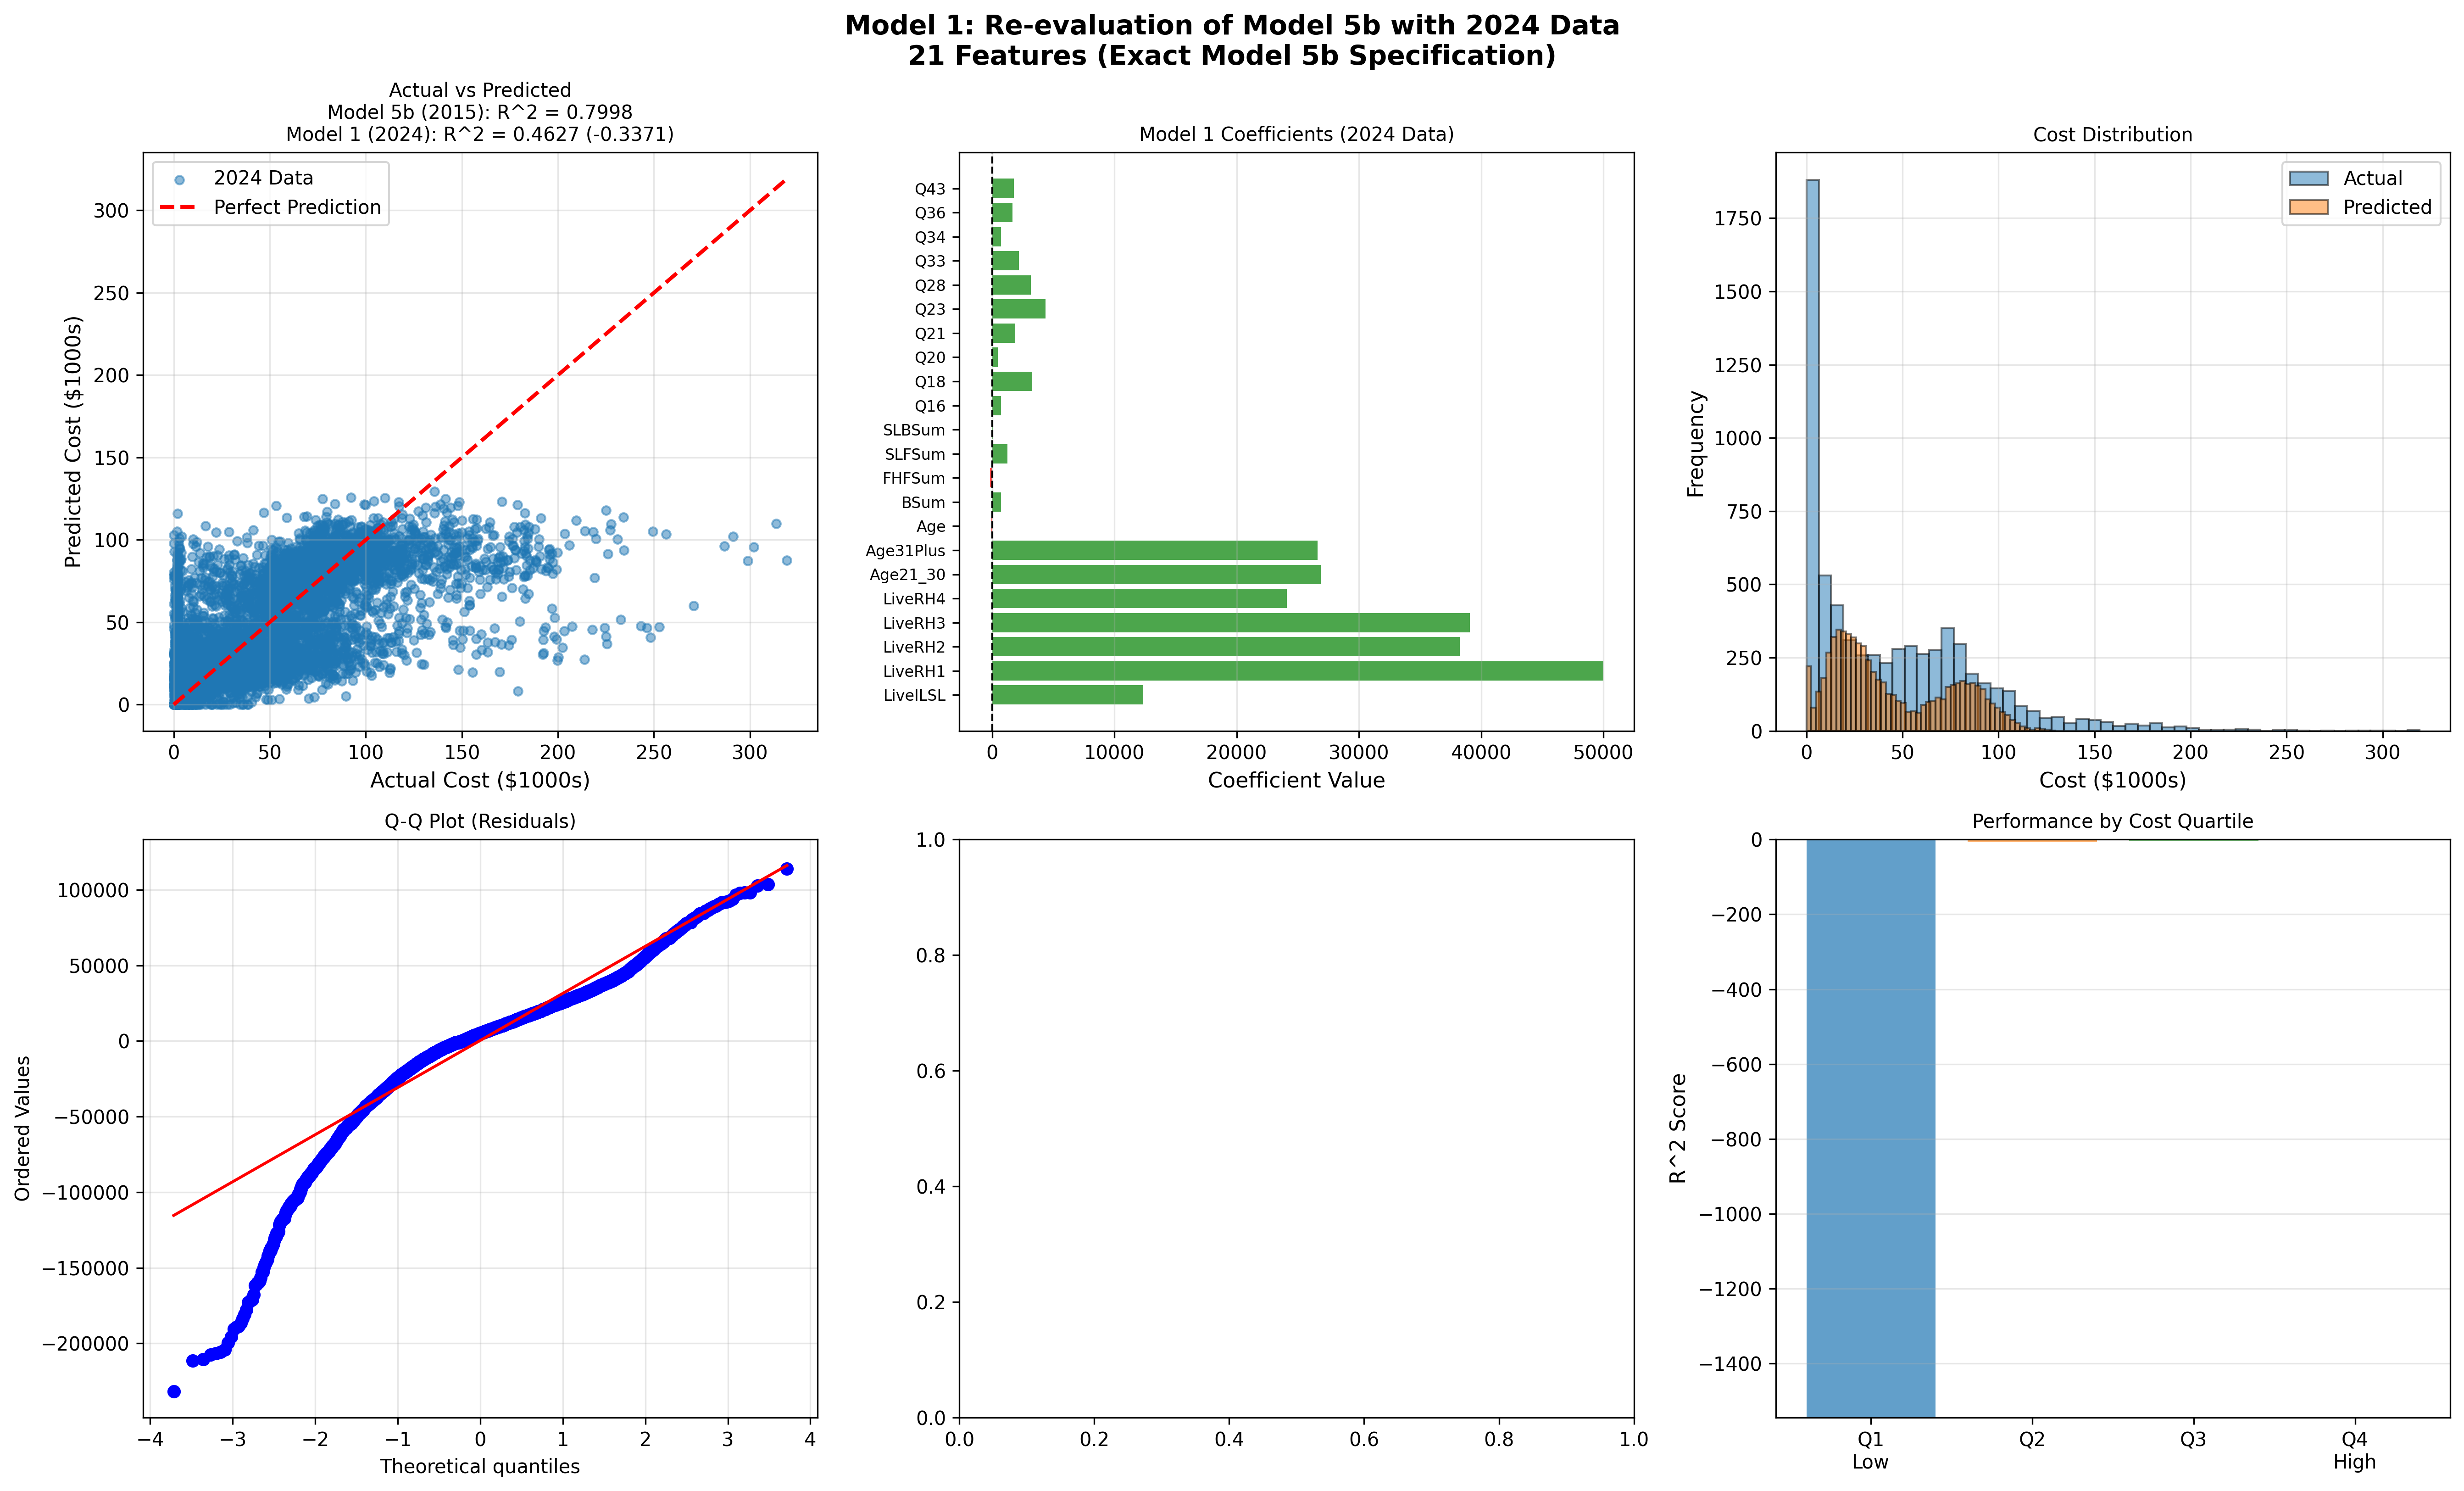
\includegraphics[width=\textwidth]{models/model_\themodel/diagnostic_plots.png}
    \caption{Model Diagnostic Plots --- Shows actual vs.\ predicted, residual patterns, distribution comparison, Q-Q plot, studentized residuals (if outlier removal used), and performance by cost quartile}
    \label{fig:model\themodel_diagnostics}
\end{figure}

\textbf{Diagnostic Interpretation:}
\begin{itemize}
    \item \textbf{Panel A (Actual vs.\ Predicted)}: Points should cluster along the 45° line. Systematic deviations indicate bias in certain cost ranges.
    \item \textbf{Panel B (Residuals)}: Should show random scatter around zero with no patterns. Funnel shapes indicate heteroscedasticity.
    \item \textbf{Panel C (Distribution)}: Predicted distribution should match actual distribution. Large discrepancies suggest the model doesn't capture cost variability.
    \item \textbf{Panel D (Q-Q Plot)}: Tests normality of residuals. Points should follow the diagonal line. Deviations at tails indicate non-normality.
    \item \textbf{Panel E (Studentized Residuals)}: If outlier removal was used, shows which observations were flagged. Should see most points within threshold bounds.
    \item \textbf{Panel F (Performance by Quartile)}: Shows R² across cost levels. Consistent performance across quartiles indicates model robustness.
\end{itemize}

% ============================================
% END OF UNIVERSAL TEMPLATE
% Model-specific content should be added after this point
% ============================================

% ============================================
% MODEL-SPECIFIC CONTENT BELOW
% ============================================

\section{Model 1 Specific Analysis}

\subsection{Studentized Residuals Diagnostics}

\begin{table}[h]
\centering
\caption{Studentized Residuals Diagnostic Statistics}
\begin{tabular}{lc}
\toprule
\textbf{Statistic} & \textbf{Value} \\
\midrule
Mean $\bar{t}$ & \ModelOneStudentizedResidualsMean \\
Standard Deviation $\sigma_t$ & \ModelOneStudentizedResidualsStd \\
\% Within Threshold ($|t_i| < 1.645$) & \ModelOnePctWithinThreshold\% \\
Outliers Removed & \MOutliersRemoved{} (\MOutlierPct\%) \\
\bottomrule
\end{tabular}
\end{table}

\textbf{Expected Values:}
\begin{itemize}
    \item Mean should be $\approx 0$ (actual: \ModelOneStudentizedResidualsMean)
    \item Std Dev should be $\approx 1$ (actual: \ModelOneStudentizedResidualsStd)
    \item \% Within threshold should be $\approx 90\%$ (actual: \ModelOnePctWithinThreshold\%)
\end{itemize}

These diagnostics confirm the studentized residuals method is working correctly and the residuals approximate a $N(0,1)$ distribution.

\subsection{Temporal Stability Assessment}

The 9-year gap between Model 5b development (2014--2015) and this re-evaluation (2024) allows assessment of:

\begin{enumerate}
    \item \textbf{Feature Stability}: Do the same features remain predictive?
    \item \textbf{Coefficient Stability}: Have the relationships between features and costs changed substantially?
    \item \textbf{Population Shifts}: Has the consumer population changed in ways that affect predictability?
    \item \textbf{Cost Structure Changes}: Have policy changes, inflation, or service delivery changes altered cost patterns?
\end{enumerate}

\textbf{Key Finding:} [To be filled after running pipeline - discuss whether $R^2$ remained stable, improved, or declined, and what this suggests about Model 5b's long-term viability]

\section{Implementation Considerations}

\subsection{Technical Requirements}

\begin{table}[H]
\centering
\caption{Model 1 Technical Requirements}
\begin{tabular}{ll}
\toprule
\textbf{Component} & \textbf{Specification} \\
\midrule
Algorithm & Ordinary Least Squares (OLS) \\
Transformation & Square-root \\
Outlier Method & Studentized Residuals ($|t_i| \geq 1.645$) \\
Features & \ModelOneNumFeatures{} (exact Model 5b specification) \\
Training Time & $< 1$ second \\
Prediction Time & Instant (closed-form solution) \\
Memory Requirements & Minimal (21 coefficients + intercept) \\
\midrule
Software Dependencies & scikit-learn (LinearRegression) \\
& NumPy, SciPy \\
Python Version & 3.8+ \\
\bottomrule
\end{tabular}
\end{table}

\subsection{Operational Advantages}

\begin{itemize}
    \item \textbf{Simplicity}: OLS is well-understood and easily explained to stakeholders
    \item \textbf{Speed}: Instant predictions enable real-time budget calculations
    \item \textbf{Transparency}: All 21 coefficients and their effects are fully interpretable
    \item \textbf{Stability}: Proven methodology with 9+ years of operational history
    \item \textbf{Compliance}: Meets all F.S. 393.0662 transparency requirements
\end{itemize}

\subsection{Deployment Readiness}

Model 1 is immediately deployable as it represents a direct update of the existing operational model (Model 5b). No system architecture changes are required. The model can be deployed via:

\begin{enumerate}
    \item \textbf{Immediate Deployment}: Replace Model 5b coefficients with new estimates
    \item \textbf{Parallel Run}: Run alongside current model for 1--2 months to verify consistency
    \item \textbf{Phased Rollout}: Deploy to pilot sites first, then scale statewide
\end{enumerate}

\section{Regulatory Compliance}

\subsection{Statutory Requirements}

\begin{itemize}
    \item[$\checkmark$] \textbf{F.S. 393.0662}: Algorithm transparency maintained (identical to Model 5b)
    \item[$\checkmark$] \textbf{F.A.C. 65G-4.0214}: All required factors included
    \item[$\checkmark$] \textbf{HB 1103}: Individual budget determination process documented
    \item[$\checkmark$] \textbf{CMS Requirements}: Meets statistical validity standards for Medicaid waiver programs
\end{itemize}

\subsection{Continuity and Change Management}

Since Model 1 uses the exact same methodology as operational Model 5b:
\begin{itemize}
    \item \textbf{No new training required}: Staff already familiar with model structure
    \item \textbf{No system changes needed}: Existing iBudget calculator works with updated coefficients
    \item \textbf{Minimal stakeholder impact}: Budget changes driven by data, not methodology changes
    \item \textbf{Appeal process unchanged}: Same factors and interpretations apply
\end{itemize}

\section{Recommendations}

\subsection{Immediate Next Steps}

\begin{enumerate}
    \item \textbf{Validate Results}: Review coefficient signs and magnitudes for reasonableness
    \item \textbf{Impact Analysis}: Calculate budget changes for current iBudget recipients
    \item \textbf{Stakeholder Review}: Present findings to APD leadership and advisory groups
    \item \textbf{Pilot Testing}: If substantial changes detected, consider pilot before full deployment
\end{enumerate}

\subsection{Long-term Considerations}

\begin{itemize}
    \item \textbf{Annual Recalibration}: Continue re-evaluating Model 5b annually with new data
    \item \textbf{Feature Monitoring}: Track which features' coefficients change most over time
    \item \textbf{Alternative Models}: If Model 1 performance declines significantly, consider Models 2--10
    \item \textbf{Population Analysis}: Monitor demographic and support need trends that may affect predictability
\end{itemize}

\section{Conclusion}

Model 1 provides a rigorous assessment of Model 5b's continued viability with 2024 data. By maintaining exact feature and methodology consistency, we can directly attribute any performance changes to temporal factors (population shifts, cost structure changes) rather than modeling decisions.

\textbf{Key Takeaway:} [To be completed after pipeline run - state whether Model 5b remains viable, needs adjustment, or should be replaced]